\section{Development}
\label{sec:development}

The \textit{development} process, building that involve coding and programming the software, is resulting the working application.
In addition, open sourcing the software source code is also done and described.

% --------------------------------------------------
\subsection{Code}

JavaScript and Meteor are used on both of the sides, while Node.js is used on the server side, all coded to implement the designed system.
JavaScript is chosen more solely because it is the primary language of the Web.
Meteor is chosen because it is heavily based on JavaScript and easy to learn than any other framework out there.
While in code development, JavaScript and CoffeeScript are both used for the logic implementation.
Below there are snippets of the code, listing \autoref{lst:satellid-code-server} is in server side and listing \autoref{lst:satellid-code-client} is in client side.
Even meteor can read all of the code in any place within the same reposutory, in actual repository however there is a convention to put the server side code into the \verb|server| folder and the client side code into the \verb|client| folder.
Both listings are intentedly to only show at a glance the upmost parts that separate each unit side.

\begin{listing}[ht]
  \caption{Satellid server side code snippets}
  \inputminted{javascript}{\dir/include/code/satellid-server.js}
  \label{lst:satellid-code-server}
\end{listing}

\begin{listing}[ht]
  \caption{Satellid client side code snippets}
  \inputminted{javascript}{\dir/include/code/satellid-client.js}
  \label{lst:satellid-code-client}
\end{listing}

\clearpage
% --------------------------------------------------
\subsection{Running and Deployment}

Running Satellid on local environment is with \verb|meteor run| command:

\begin{listing}[h]
\caption{Running Meteor app locally}
\inputminted{shell-session}{\dir/include/satellid-meteor-run.shell-session}
\label{lst:satellid-run}
\end{listing}

Deploying Satellid to the Internet with Meteor is with the following \verb|meteor deploy appname.meteor.com| command:

\begin{listing}[h]
\caption{Deploying Meteor app}
\inputminted{shell-session}{\dir/include/satellid-meteor-deploy.shell-session}
\label{lst:satellid-deploy}
\end{listing}

After this, the application result is live and available at \url{http://satellid.meteor.com}.

% --------------------------------------------------
\subsection{Result}

The screenshot of final result is like in \autoref{fig:satellid-app-result}.
Then each of the results of \ac{BREAD} feature or operation, are like in
\autoref{fig:satellid-app-results_read},
\autoref{fig:satellid-app-results_browse},
\autoref{fig:satellid-app-results_add},
\autoref{fig:satellid-app-results_edit}, and
\autoref{fig:satellid-app-results_delete}

\begin{figure}[!htp]
  \centering
  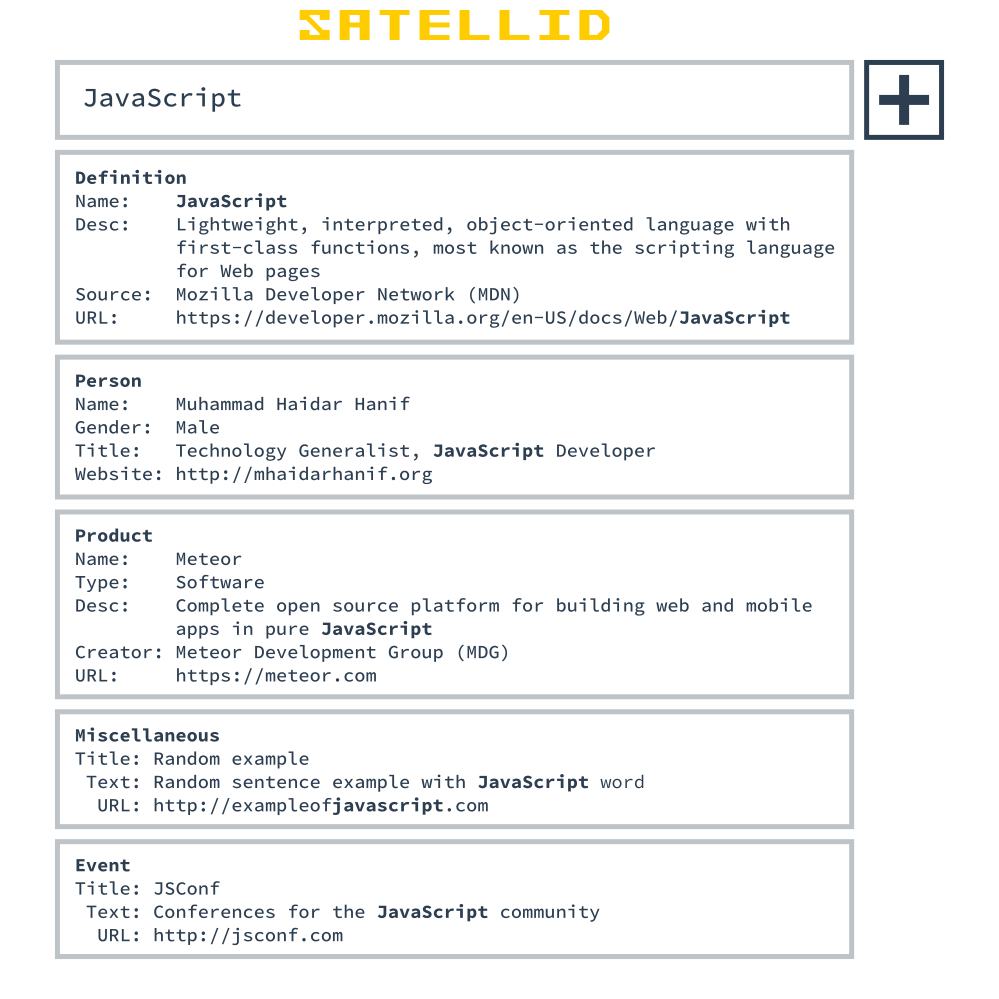
\includegraphics[width=\textwidth]{\dir/include/satellid-app-result.png}
  \caption{Final app screenshot of the development result}
  \label{fig:satellid-app-result}
\end{figure}

\begin{figure}[!htp]
  \centering
  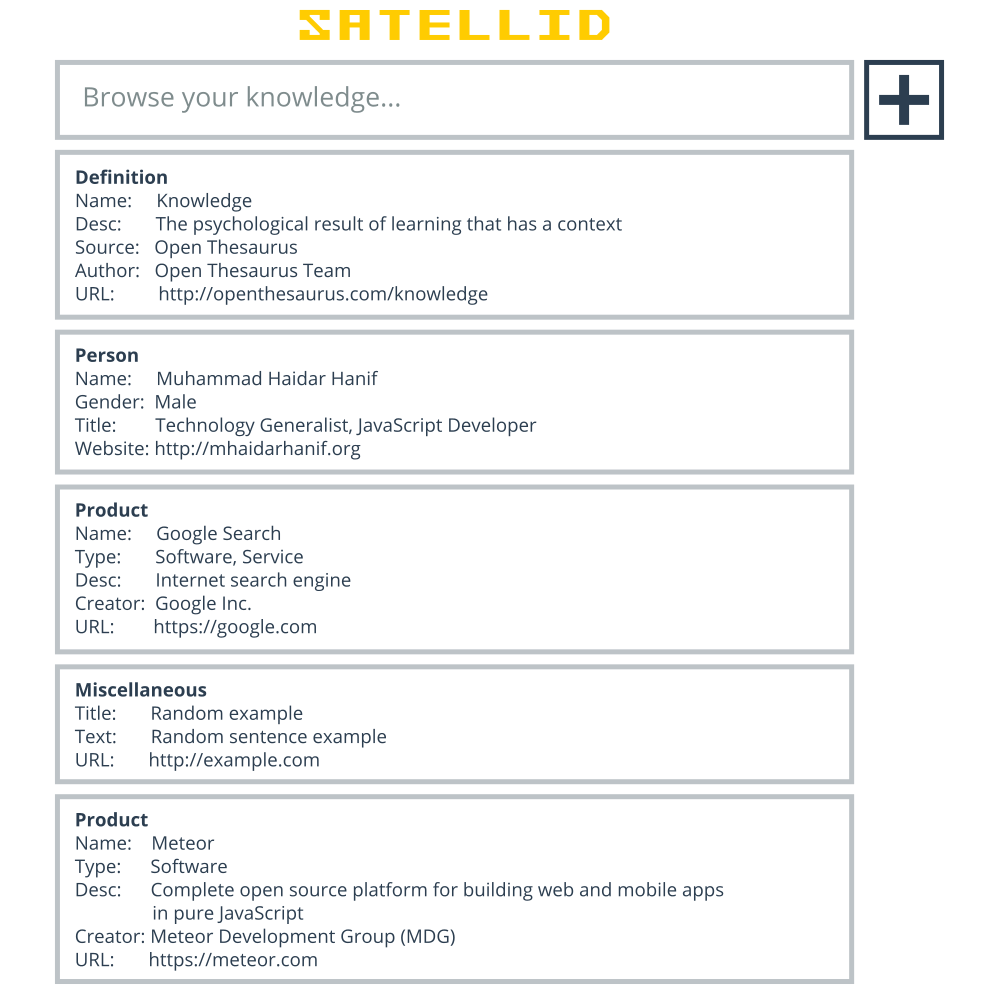
\includegraphics[height=10cm]{\dir/include/satellid-app-results_read.png}
  \caption{Screenshot of READ interaction}
  \label{fig:satellid-app-results_read}
\end{figure}

\begin{figure}[!htp]
  \centering
  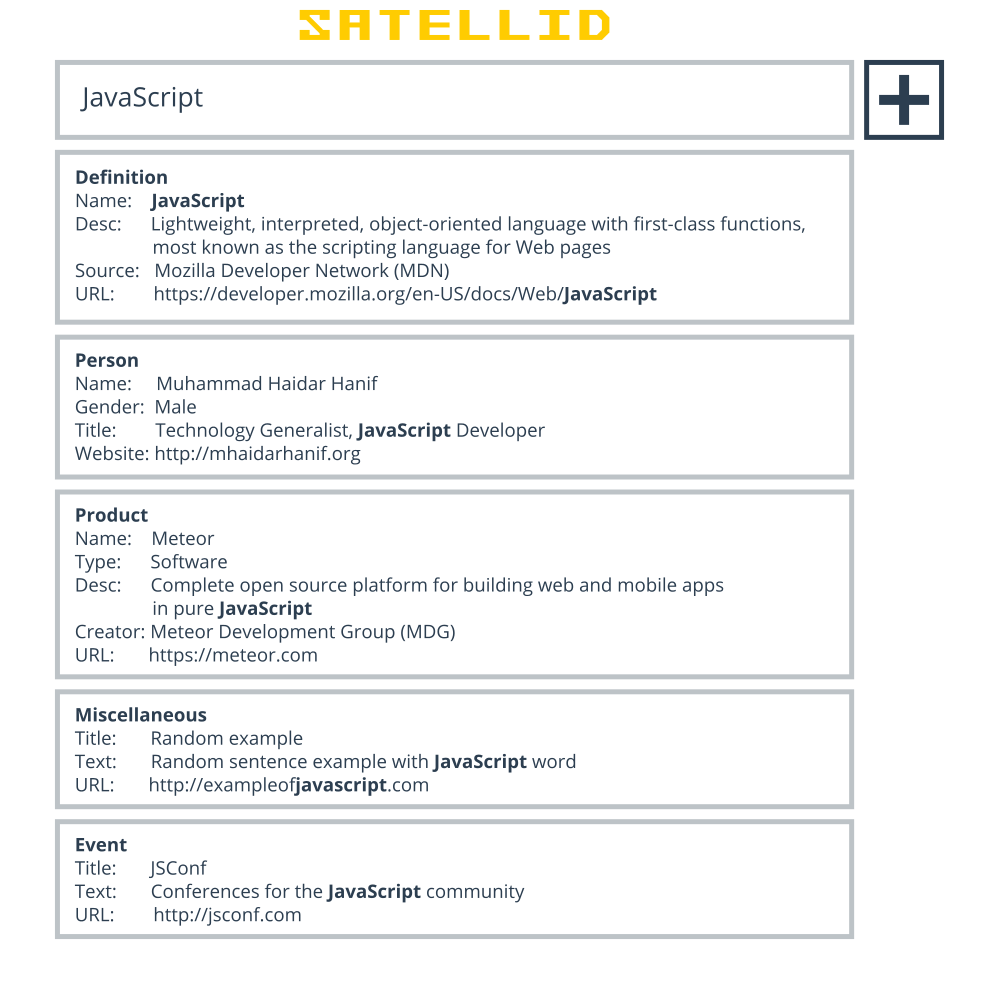
\includegraphics[height=10cm]{\dir/include/satellid-app-results_browse.png}
  \caption{Screenshot of BROWSE interaction}
  \label{fig:satellid-app-results_browse}
\end{figure}

\begin{figure}[!htp]
  \centering
  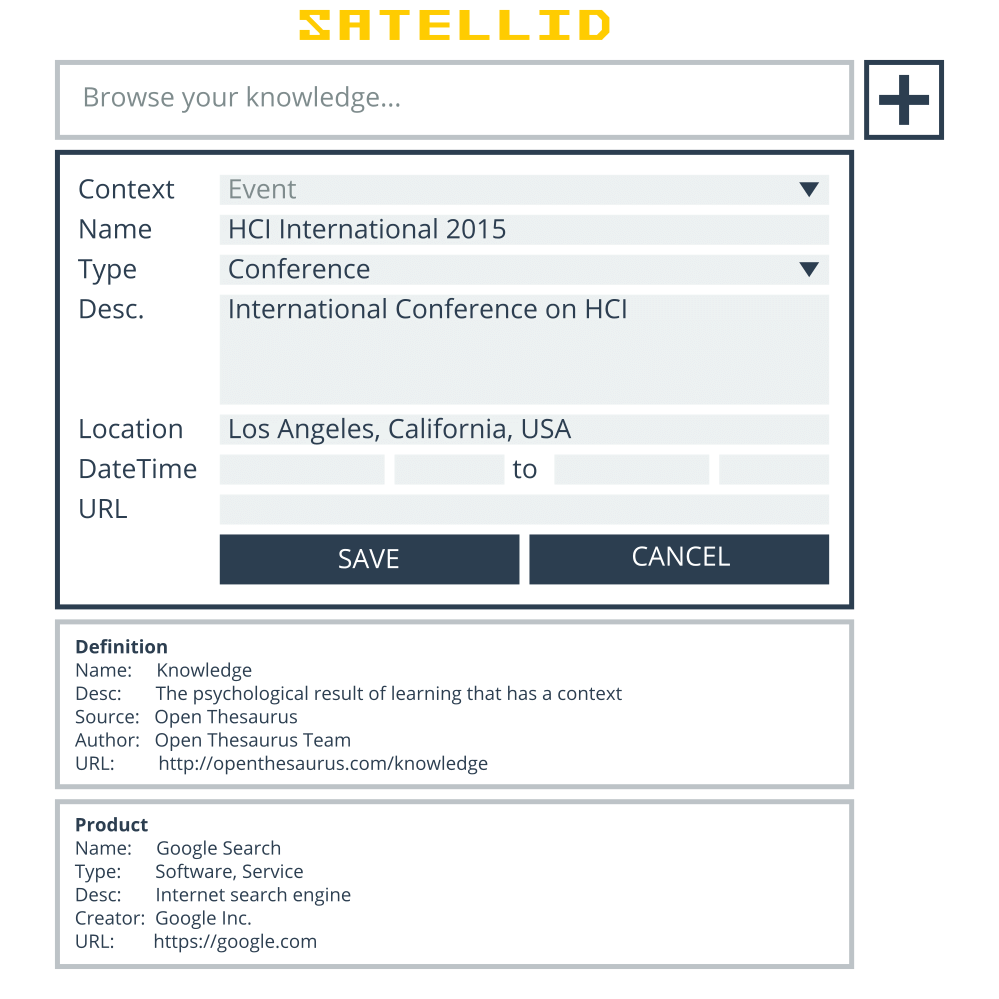
\includegraphics[height=10cm]{\dir/include/satellid-app-results_add.png}
  \caption{Screenshot of ADD interaction}
  \label{fig:satellid-app-results_add}
\end{figure}

\begin{figure}[!htp]
  \centering
  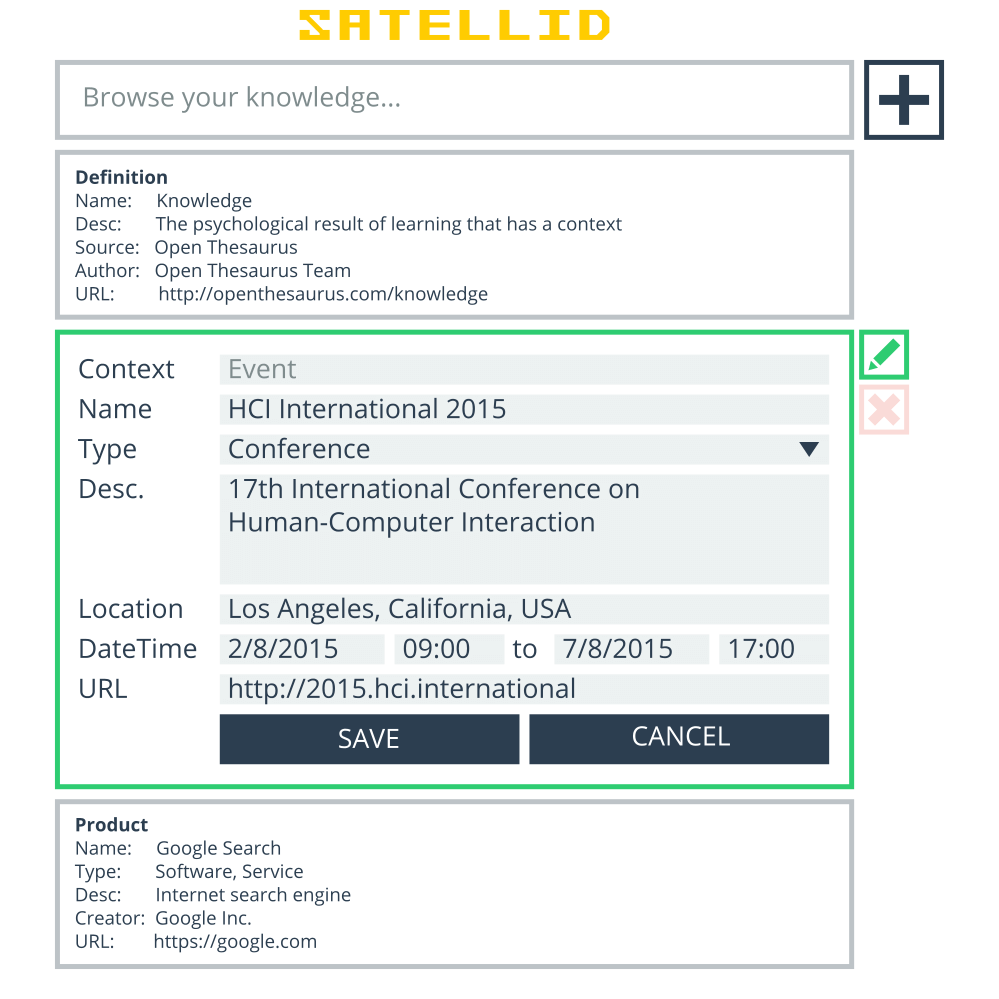
\includegraphics[height=10cm]{\dir/include/satellid-app-results_edit.png}
  \caption{Screenshot of EDIT interaction}
  \label{fig:satellid-app-results_edit}
\end{figure}

\begin{figure}[!htp]
  \centering
  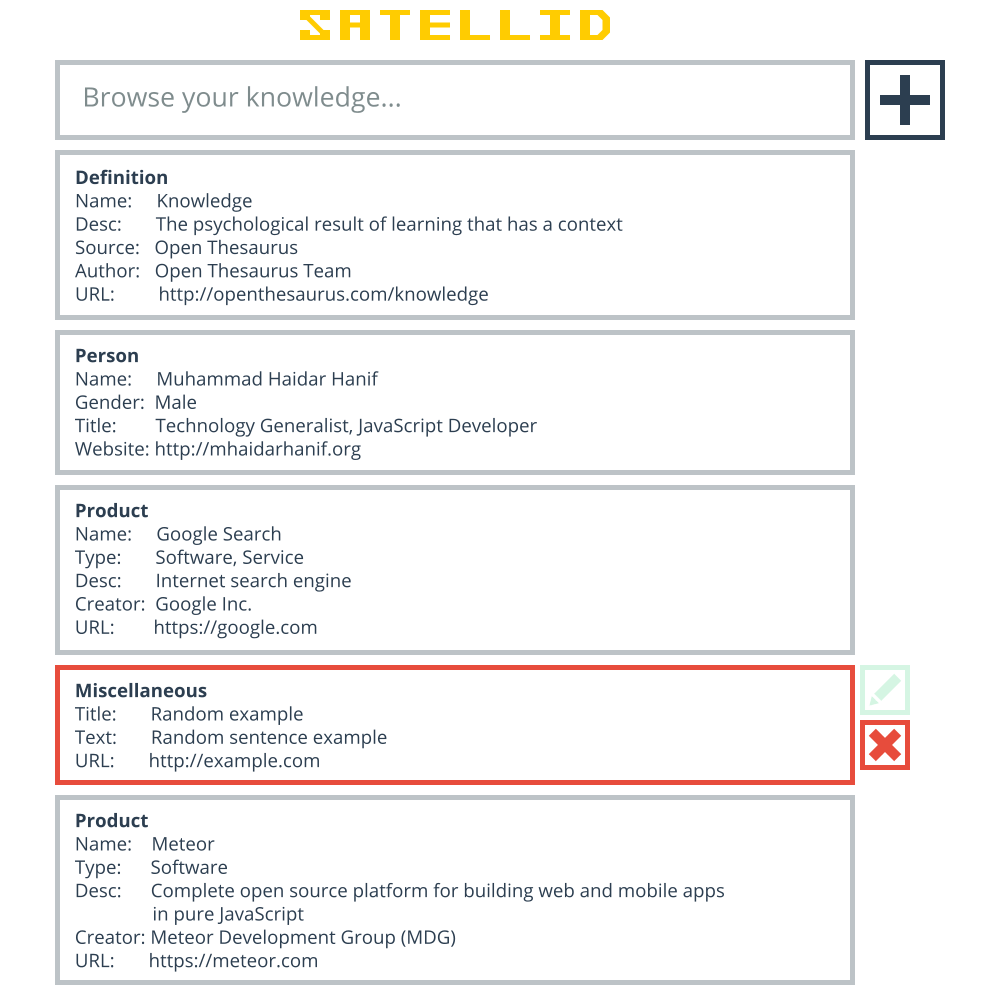
\includegraphics[height=10cm]{\dir/include/satellid-app-results_delete.png}
  \caption{Screenshot of DELETE interaction}
  \label{fig:satellid-app-results_delete}
\end{figure}


% --------------------------------------------------
\subsection{Open Sourcing}

Below in listing \autoref{lst:git} is a process of creating a Git\index{Git} repository\index{repository} and releasing it as an open source\index{open source} project.
All done within terminal/\ac{CLI} and the utilization of Git \ac{SCM}.

\begin{listing}[!h]
\caption{Committing and pushing the repo with Git}
\inputminted{shell-session}{\dir/include/git.shell-session}
\label{lst:git}
\end{listing}

The repository is first initialized as a Git repository.
Then all the files are added and committed with a message.
Lastly, a remote \ac{URL} of the repository on the Web is added then pushed to there.
In this process, now the Satellid repository is available at GitHub\index{GitHub} with \ac{URL} \url{https://github.com/satellid/satelid-meteor}, as a public repository or open source project.
